\label{cha:analyse}
Für die Konzeption und Implementierung des Moodle-Plugins ist zunächst eine Analyse. In der Analyse sollen basierend auf der Zielgruppe Anforderungen an das Plugin zu bestimmt und priorisiert werden. Darauf aufbauend wird, nach kurzer Betrachtung der Möglichkeiten bei der Moodle Plugin-Entwicklung, der aktuelle Stand der Technik betrachtet.

%\begin{figure}[h!]
%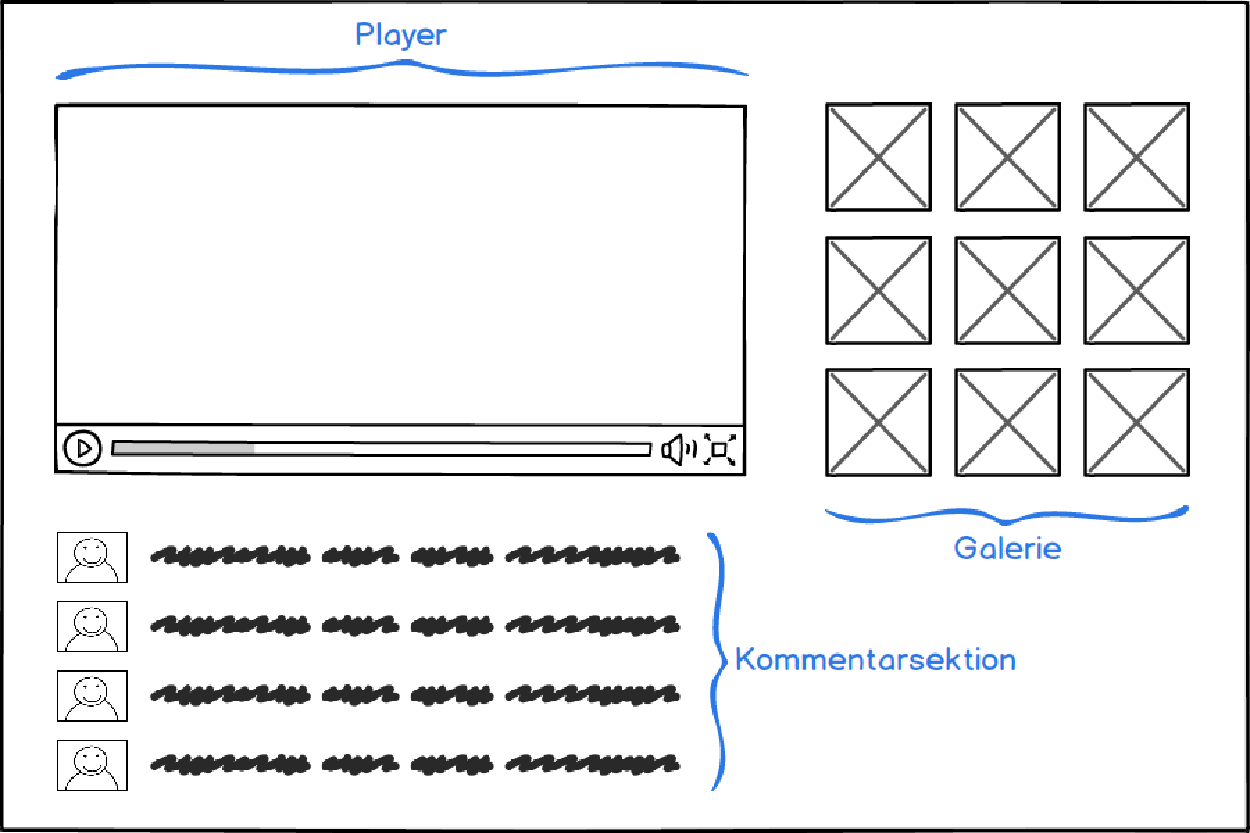
\includegraphics[width=.8\textwidth,center]{MockupBereiche.pdf}
%\caption{\label{fig:MockupBereiche}Erste Skizze der Moodle-Repräsentation eines Hyperaudio-Dokuments}
%\end{figure}

\todo[inline]{Einleitung erweitern}

%%%%%%%%%%
\section{Zielgruppe}
Im nächsten Schritt soll die Zielgruppe anhand von \textit{Personas} und deren \textit{User Stories} festgelegt werden. Dies soll dann die Grundlage für die Definition der Anforderungen im nächsten Abschnitt darstellen.

\todo[inline]{Einleitung erweitern}

%%%%%%%%%%
\subsection{Personas}
\label{sec:personas}
%https://dl.gi.de/bitstream/handle/20.500.12116/5888/Holt_Winter_Thomaschewski_2011.pdf?sequence=2
Bevor sich den \textit{User Stories} zugewendet werden kann, müssen vorab die dafür nötigen \textit{Personas} entwickelt werden. Unter \textit{Personas} werden fiktive Benutzer verstanden, für welche das Programm, in unserem Fall das Moodle-Plugin, designt wird \citep{cooper2004inmates}. Jeder Persona wird eine Rolle im Zusammenhang mit der Anwendung zugewiesen. Darüber hinaus wird die Persona ausreichend beschrieben, damit sich leicht in die Person hineinversetzt werden kann \citep{cohn2004user}. Dieses Vorgehen hilft dabei, möglichst authentische \textit{User Stories} zu generieren, ohne auf echte Benutzer zurückgreifen zu müssen.

\todo[inline]{Die Personas sind ein guter Anfang. Beschreiben Sie die Lebenssituation der Studierenden noch besser. Zeigen Sie auf, wann die Leute etwa Pendeln, Autofahren oder unbezahlte Arbeit daheim verrichten. }



\par
\begingroup
\leftskip=1cm
\rightskip=1.5cm
\noindent

{\Large\emph{Prof. Dr. Karolin Schröder}} ist verantwortlich für den Kurs \glqq Einführung in die Wirtschaftsinformatik\grqq{}. In diesem Kurs werden bereits erfolgreich Hyperaudio-Dokumente eingesetzt. Nachdem Prof. Dr. Schröder mit dem Start des nächsten Semesters überarbeitete Kurseinheiten anbietet, müssen nun auch die vorhandenen Hyperaudio-Dokumente auf die Notwendigkeit einer Überarbeitung hin überprüft werden. Die veralteten Hyperaudio-Dokumente müssen dann durch neuere Versionen ersetzt werden.
\vspace{.5cm}

{\Large\emph{Dr. Julian Schmidt}} ist wissenschaftlicher Mitarbeiter und Betreuer für den Kurs \glqq Marketing\grqq{}. Nachdem der Kurs auch das Lernen mittels Hyperaudio-Dokument anbietet, ist er unter anderem für die Betreuung dieser verantwortlich und ist derjenige, der hier Rede und Antwort steht.
\vspace{.5cm}

{\Large\emph{Laura Ebert}} \textbf{ist 35 Jahre alt, verheiratet und hat drei Kinder. Sie geht halbtags einem Beruf nach, zu dem sie 30 Minuten mit dem Bus pendelt. Neben der Arbeit kümmert sie sich zusammen mit ihrem Mann um den Haushalt und die Kinder. Laura studiert in Teilzeit den Bachelorstudiengang Informatik im ersten Semester.} Das Semester hat erst vor einigen Wochen begonnen und sie entdeckt gerade Moodle für sich. Hierbei ist sie auf die Hyperaudio-Dokumente gestoßen und hat sich fest vorgenommen, sich im Laufe des Semsters mit deren Hilfe mit den Lerninhalten auseinanderzusetzen.
\vspace{.5cm}
 
{\Large\emph{Max Lustig}} \textbf{ist 24 Jahre alt, ledig und hat sich nach einer abgeschlossenen Ausbildung dazu entschlossen, neben dem Beruf zu studieren. Sein Berufsweg besteht aus einem 20 minütigen Gang zu Fuß. Neben der Arbeit ist Max ein begeistertet Fitnessstudiogänger.} Er absolviert ein Vollzeitbachelorstudium in Wirtschaftsinformatik und befindet sich kurz vor der Prüfungsphase zum Ende des dritten Semesters. Max möchte sich nun auf die Klausur des Moduls \glqq Investition und Finanzierung (BWL II)\grqq{}, welche in zwei Wochen stattfindet, intensiv vorbereiten. Im Laufe des Semsters hat er bereits ausgiebig die neuen Hyperaudio-Dokumente zum Erreichen des Lernziels genutzt.

\par
\endgroup

%%%%%%%%%%
\subsection{User Stories}
\textit{User Stories} beschreiben, wie die klassischen \textit{Use Cases}, Anforderungen an ein Softwaresystem. Diese sind dabei im Vergleich wesentlich oberflächlicher und ungenauer formuliert als \textit{Use Cases} \citep{wirdemann2017scrum}.

Erst im Laufe der Entwicklung werden \textit{User Stories} konkreter und dienen am Ende dazu deren Ergebnis zu validieren. Beim Erstellen von \textit{User Stories} ist zu beachten, dass sogenannte \textit{Epics}, das sind \textit{User Stories} mit sehr großem Umfang, wenn möglich in kleinere \textit{User Stories} aufgesplittet werden. Unter anderem ist zu beachten, dass die \textit{User Stories} keine Abhängigkeiten untereinander aufweisen und dass deren Erfüllung überprüfbar ist. \textit{User Stories} können im \textit{Connextra Format} festgehalten werden, welches wie folgt aufgebaut ist \citep{cohn2004user}:

\par
\begingroup
\leftskip=1cm
\rightskip=1.5cm
\noindent

\textit{Ich als (Rolle) möchte (Funktion), um (Nutzen).}

\par
\endgroup

\vspace{.3cm}

Mit den Unterschieden und Einsatzzwecken von Personas und Rollen beschäftigt sich \cite{constantine2006users}. Grundsätzlich ist demnach festzustellen, dass Personas eher aus dem \textit{User-centered design} \citep{Norman1986user}, Benutzerrollen dagegen aus dem \textit{Usage-centered design} \citep{Constantine1996usage} motiviert sind. Während sowohl Personas als auch Benutzerrollen durchaus nützlich sind, um ein Verständnis von den Nutzern eines Systems zu erhalten, unterscheiden sie sich nach \cite{constantine2006users} in ihrer Philosophie und Relevanz für das Interaktionsdesign. Im Gegensatz zu Personas, die wie bereits im vorangegangenen Abschnitt \ref{sec:personas} beschrieben dazu dienen, die Nutzersicht anhand möglichst realer Personen darzustellen, sollen Benutzerrollen in einer wesentlich technischeren Sicht ein abstrahiertes Modell für die Art und Weise, in der Nutzer mit dem System interagieren, bilden \citep{constantine2006users}.

Für die weitere Analyse soll das Beste beider Welten vereinbart werden. Um die \textit{User Stories} möglichst anschaulich zu halten, werden sie anhand der vorgestellten Personas definiert. Gleichzeitig wird eine Aufteilung in Benutzerrollen vorgenommen, die die Grundlage für die Ableitung von Anforderungen aus den \textit{User Stories} bildet.

Für die Konzeption des Moodle-Plugins ergeben sich im Wesentlichen zwei Benutzerrollen wie in Abbildung \ref{fig:Rollen} dargestellt. \textit{Administrierende} sind diejenigen Anwender, die Lerninhalte in Form von Hyperaudio-Dokumenten bereitstellen und verwalten. Diese Rolle kann nur von Lehrenden eingenommen werden. Die Gruppe der \textit{Nutzenden} kann derweil aus Lehrenden sowie Studierenden bestehen, die mit Hyperaudio-Dokumenten interagieren möchten.

\begin{figure}[h!]
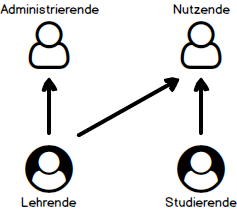
\includegraphics[width=.3\textwidth,center]{Rollen.png}
\caption{\label{fig:Rollen}Benutzerrollen}
\end{figure}


Für das Angebot einer alternativen Repräsentation von Lerninhalten als Hyperaudio-Dokumente lassen sich folgende \textit{User Stories} festhalten.

\todo[inline]{Sehr gut. Es gibt natürlich noch dutzende User Storys. Versuchen Sie die Storys gleich zu nummerieren. Anschließend können Sie die Nummer einzelnen Komponenten zuordnen und dann gebündelt bearbeiten. Feature: Sie können Stories natürlich auch mit der Zielgruppe zusammen entwickeln oder diese bewerten lassen. Somit hätten Sie eine Absicherung, nicht am Nutzer vorbei zu entwickeln. 
}
\todo[inline]{Lehrend möchten außerdem den Inhalt ihrer bestehenden Kurse vollständig als Audio/Hyperaudio abbilden können. Formeln, Tabellen, Bilder, ...
Sie möchten bei der Konvertierung/Produktion wenig arebeit haben. Sie möchten Inhalte nachträglich editieren (auch Audio?!). }


\begin{enumerate}

\item Als Administrierende möchte Prof. Dr. Karolin Schröder ein neues Hyperaudio-Dokument in ihrem Kurs \glqq Einführung in die Wirtschaftsinformatik\grqq{} zur Verfügung stellen, um den Studierenden neue Lerninhalte bereitzustellen.

\item Als Administrierende möchte Prof. Dr. Karolin Schröder Hyperaudio-Dokumente aus ihrem Kurs \glqq Einführung in die Wirtschaftsinformatik\grqq{} löschen können, um veraltete Informationen zu entfernen.

\item Als Administrierende möchte Prof. Dr. Karolin Schröder Hyperaudio-Dokumente aus ihrem Kurs \glqq Einführung in die Wirtschaftsinformatik\grqq{} im Sommersemester in den darauffolgenden Kurs im Wintersemester übernehmen\textbf{, um diese nicht erneut hochladen zu müssen.}

\item Als Administrierende möchte Prof. Dr. Karolin Schröder Hyperaudio-Dokumente anderer Kurse in ihren Kurs \glqq Einführung in die Wirtschaftsinformatik\grqq{} übernehmen\textbf{, um sich nicht selbst die Arbeit machen zu müssen, da sich die Themen mit ihrem Kurs überschneiden und wiederverwendet werden können.}

\item Als Administrierende möchte Prof. Dr. Karolin Schröder Erkenntnisse daraus gewinnen, wie die Hyperaudio-Dokumente des Kurses \glqq Einführung in die Wirtschaftsinformatik\grqq{} von Studierenden genutzt werden, um Verbesserungspotenzial auszumachen.

\item Als Administrierender möchte Dr. Julian Schmidt ein vorhandenes Hyperaudio-Dokument in dem von ihm betreuten Kurs \glqq Marketing\grqq{} überarbeiten, um einen Fehler zu beseitigen.

\item Als Nutzende möchte Prof. Dr. Karolin Schröder die bereits vorhandenen Hyperaudio-Dokumente aus ihrem Kurs \glqq Einführung in die Wirtschaftsinformatik\grqq{} wiedergeben, um diese auf ihre Richtigkeit zu überprüfen.

\item Als Nutzende möchte Prof. Dr. Karolin Schröder die Kommentare zu einem Hyperaudio-Dokument lesen und beantworten können, um auf Fragen von Studierenden einzugehen.

\item Als Nutzende möchte Prof. Dr. Karolin Schröder eine Notiz zu einem Hyperaudio-Dokument machen, um ihren Gedanken festzuhalten und später darauf zurückgreifen zu können.

\item Als Nutzender möchte Dr. Julian Schmidt eine gefundene Erklärungslücke in einem Hyperaudio-Dokument durch einen Kommentar zum entsprechenden Zeitpunkt schließen.

%\item \textit{Dr. Julian Schmidt stellt eine Erklärungslücke in einem Hyperaudio-Dokument fest und möchte diese durch einen Kommentar zum entsprechenden Zeitpunkt schließen.}

\item \textbf{Als Nutzende möchte Laura Ebert mittels Hyperaudio-Dokument lernen, um die Zeit während Haushaltsarbeiten, wie dem Bügeln, Kochen oder Putzen, und dem Pendeln sinnvoller zu nutzen.}

\item Als Nutzende möchte Laura Ebert erfahren, welche Hyperaudio-Dokumente in den von ihr belegten Kursen angeboten werden.

\item Als Nutzende möchte Laura Ebert einen Kommentar verfassen, um dem Kursbetreuer und den anderen Studierenden eine Frage zu stellen.

\item Als Nutzende möchte Laura Ebert eine Markierung setzen, wenn eine klausurrelevante Thematik erklärt wird. Bei der Prüfungsvorbereitung möchte sie anhand dieser Markierungen diejenigen Themen erkennen, mit welchen sie sich besonders intensiv beschäftigen möchte.

\item Als Nutzende möchte Laura Ebert eine Markierung löschen, da sie den markierten Lerninhalt inzwischen beherrscht. Anhand der übrigen Markierungen möchte sie schnell erkennen, wo für sie noch Lernbedarf besteht.

\item Als Nutzende möchte Laura Ebert eine Notiz erstellen, um ein Beispiel zu dem genannten Sachverhalt festzuhalten, sodass sie die Thematik beim nächsten Mal einfacher nachvollziehen kann.

\item Als Nutzende möchte Laura Ebert die Wiedergabe eines Hyperaudio-Dokuments beenden und am nächsten Tag an derselben Stelle fortsetzen.

\item Als Nutzende möchte Laura Ebert die Hyperaudio-Angebote auch unterwegs mit ihrem Smartphone in Anspruch nehmen.

\item Als Nutzender möchte Max Lustig eine alte Notiz bearbeiten, um einen Schreibfehler zu korrigieren.

\item Als Nutzender möchte Max Lustig eine alte Notiz löschen, da er inzwischen Lernfortschritte gemacht hat und auf diese Notiz verzichten kann.

\item Als Nutzender möchte Max Lustig nach Inhalten in Hyperaudio-Dokumenten suchen können, um schneller das Hyperaudio-Dokument zu finden, in dem ein bestimmtes Thema behandelt wird.

\item Als Nutzender möchte Max Lustig nach Textinhalten in Kommentaren suchen können, um schnell Erklärungen zu finden.

\item Als Nutzender möchte Max Lustig auf Kommentare antworten können, um sich mit den Studierenden und Lehrenden auszutauschen.

\item Als Nutzender möchte Max Lustig erkennen, welche Hyperaudio-Dokumente er zuletzt abgespielt hat, um seinen Lernfortschritt im Auge zu behalten.

\item Als Nutzender möchte Max Lustig besonders hilfreiche Hyperaudio-Dokumente als Favoriten speichern, um diese schnell als solche identifizieren zu können.

\item Als Nutzender möchte Max Lustig die Markierung als Favorit entfernen können, wenn es für ihn nicht mehr von Interesse ist.

\end{enumerate}




%%%%%%%%%%
\subsection{Umgebungsbedingungen}
\todo[inline]{Rahmen in dem das Plugin durch Studierende genutzt werden können soll}

%%%%%%%%%%
\section{Anforderungsdefinition}
\label{sec:anforderungsdefinition}
Basierend auf den \textit{Personas}, deren Rollen und deren \textit{User Stories} können nun die Andorderungen für das Moodle-Plugin definiert werden. Hierbei wird aus einer oder mehreren \textit{User Stories} jeweils eine oder mehrere Anforderungen abgeleitet und im gleichen Schritt mit einer Priorität versehen. Für die Priorisierung stehen die drei Prioritätsstufen \textit{niedrig}, \textit{mittel} und \textit{hoch} zur Verfügung. Bei der Priorisierung der Anforderungen soll die Zielsetzung aus \ref{cha:einfuehrung} als Grundlage dienen.

%%%%%%%%%%
\subsection{Anforderungen der Administrierenden}
Es wird mit der Definition der Anforderungen der Administrierenden begonnen, diese werden in der Tabelle \ref{tab:AnforderungenAdministrierenden} festgehalten.

Aus \textit{User Story}:1 kann die Anforderung zum Erstellen von Hyperaudio-Dokumenten abgeleitet werden. Dies stellt eine der Grundfunktionalitäten für die alternative Repräsentation der Lerninhalte dar und wird dementsprechend mit \textit{hoch} bewertet.

Die Anforderung bestehende Hyperaudio-Dokumente bearbeiten zu können entsteht aus \textit{User Story}:6,  
\todo[inline]{Priorisierung}

Das Löschen von Hyperaudio-Dokumenten wird durch \textit{User Story}:2 als Anforderung festgelegt,
\todo[inline]{Priorisierung}

Mit \textit{User Story}:3 und \textit{User Story}:4 ergibt sich die Anforderung, dass Hyperaudio-Dokumente in einen anderen Kurs übernommen werden können sollen, sei es der gleiche Krus im nächsten Semester oder ein komplett anderer Kurs.
\todo[inline]{Priorisierung}

Der Wunsch Erkenntnisse aus der Nutzung von Hyperaudio-Dokumenten durch die Studierenden zu erhalten, schlägt sich in der Anforderung nach statistischen Auswertungsmöglichkeiten nieder.
\todo[inline]{Priorisierung}
\todo[inline]{Fertigstellen}

\begin{table}[!ht]
\def\arraystretch{1.4}
\caption{Anforderungen der Administrierenden}
\label{tab:AnforderungenAdministrierenden}
 \begin{tabularx}{\textwidth}{lXll}      
    \hline
    Nr. & Anforderung & Priorität
    \\\hline
    1 & Erstellen eines Hyperaudio-Dokuments & hoch\\
    2 & Bearbeiten eines Hyperaudio-Dokuments & mittel\\
    3 & Löschen eines Hyperaudio-Dokuments & mittel\\
    4 & Übernahme eines Hyperaudio-Dokuments in einen anderen Kurs & mittel\\
    5 & Statistische Auswertungen über die Nutzung der Hyperaudio-Dokumente & niedrig\\
    \hline
    \end{tabularx}
\end{table}


%%%%%%%%%%
\subsection{Anforderungen der Nutzenden}
Bei den Anforderungen der Nutzenden wird wie im vorangegangen Abschnitt vorgegangen. Die Ergebnisse werden in der Tabelle \ref{tab:AnforderungenNutzenden} festgehalten.

Aus \textit{User Story}:7 und \textit{User Story}:11 ergibt sich die Andorderung, Hyperaudio-Dokumente abspielen zu können, was eine Grundfunktion des Plugins darstellt und somit mit \textit{hoch} bewertet wird. Aus \textit{User Story}:11 ergibt sich zusätzlich die Anforderung an \textit{Audio Cues} (siehe Abschnitt \ref{sec:audiocues}) mittels denen auf annotierte Zusatzinhalte hingewiesen wird. Nur dadurch, ist das Ziel der größeren zeitlichen Flexibilität beim Lernen erreichbar. Aus diesem Grund wird dieser Anforderung ebenfalls die Prioritätsstufe \textit{hoch} zugewiesen.

\todo[inline]{Übersicht über annotierte Zusatzinhalte}

Basierend auf \textit{User Story}:8, \textit{User Story}:10, \textit{User Story}:13 und \textit{User Story}:23 entstehen die Anforderungen an eine Kommentarfunktion mit den Möglichkeiten zum Erstellen, Anzeigen und Beantworten von Kommentaren. Da dies ein zentraler Aspekt für die gewünschte Kooperation unter Studierenden und den Lehrenden darstellt werden diese Anforderungen alle mit \textit{hoch} bewertet. Der aus \textit{User Story}:23 stammenden Anforderung nach einer Suchfunktion wird hingegen nur eine niedrige Priorität zugewiesen, da diese im Vergleich zu den anderen Anforderungen nur wenig zum erreichen der gesetzten Ziele beiträgt.

In \textit{User Story}:9, \textit{User Story}:16, \textit{User Story}:19 und \textit{User Story}:20 werden Wünsche bezüglich einer Notizfunktion formuliert. Hieraus resultieren die Anforderungen persönliche Notizen erstellen, anzeigen, bearbeiten und löschen zu können. Diese Anforderung spiegelt das Ziel der Erhaltung typischer Nutzerinteraktionen mit textuellen Lernmedien wieder und kann das Lernen für die Studierenden erleichtern \citep{scutter2010students}. In diesem Sinne wird auch dem Erstellen und Anzeigen eine hohe Priorität zugewiesen, dem Ändern und Löschen wiederum nur eine mittlere.

Ähnlich sind die Anforderung zum Erstellen , Anzeigen und Löschen von persönlichen Markierungen aus \textit{User Story}:14 und \textit{User Story}:15 zu bewerten. Da es sich hierbei nur um eine abgespeckte Form von persönlichen Notizen handelt, werden diese aber durchweg eine Prioritätsstufe  niedriger bewertet.

Ein Wunsch nach einer Favoritenfunktion für Hyperaudio-Dokumente ergibt sich wiederum aus \textit{User Story}:25 und \textit{User Story}:26. Dieser Wunsch resultiert in der Anforderung Favoriten setzten, anzeigen und löschen zu können.
\todo[inline]{Priorisierung}

Aus \textit{User Story}:12 und \textit{User Story}:24 ergibt sich jeweils eine Anforderung nach einer Übersicht. Im ersten Fall eine Übersicht über alle Hyperaudio-Dokumente der belegten Kurse und im zweiten Fall eine Übersicht über die zuletzt abgespielten Hyperaudio-Dokumente. Beide Anforderungen stellen nur eine reine Optimierung der Navigation dar und verhelfen somit nur indirekt der Zielerreichung. Somit erhalten sie die Bewertung \textit{niedrig}.

Eine Anforderung für eine Funktion zum Fortsetzen unterbrochener Wiedergaben bei folgenden Aufrufen in Moodle ergibt sich aus \textit{User Story}:17.
\todo[inline]{Priorisierung}

Das Verlangen Hyperaduio-Dokumente, wie in \textit{User Story}:18 beschrieben, auch auf einem Smartphone verwenden zu können, resultiert in der Anforderung zur Unterstützung von mobilen Endgeräten.
\todo[inline]{Priorisierung}

\todo[inline]{Fertigstellen}

\begin{table}[!ht]
\def\arraystretch{1.4}
\caption{Anforderungen der Nutzenden}
\label{tab:AnforderungenNutzenden}
\begin{tabularx}{\textwidth}{lXll}      
    \hline
    Nr. & Anforderung & Priorität
    \\\hline
    1 & Wiedergabe von Hyperaudio-Dokumenten & hoch\\
    2 & Hinweise auf die Darstellung von annotierten Zusatzinhalten & hoch\\
    3 & Übersicht über annotierte Zusatzinhalte & mittel\\
    4 & Kommentarfunktion bei Hyperaudio-Dokumenten & \\
    4.1 & Erstellen von Kommentaren & hoch\\
    4.2 & Anzeigen von Kommentaren & hoch\\
    4.3 & Antworten von Kommentaren & hoch\\
    4.4 & Suchfunktion innerhalb der Kommentare & niedrig\\ 
    5 & Notizfunktion bei Hyperaudio-Dokumenten & \\
    5.1 & Erstellen von Notizen & hoch\\
    5.2 & Anzeigen von Notizen & hoch\\
    5.3 & Bearbeiten von Notizen & mittel\\
   	5.4 & Löschen von Notizen & mittel\\
    6 & Markierungsfunktion bei Hyperaudio-Dokumenten & \\
    6.1 & Erstellen von Markierungen & mittel\\
    6.2 & Anzeigen von Markierungen & mittel\\
   	6.3 & Löschen von Markierungen & niedrig\\
    7 & Favoritenfunktion für Hyperaudio-Dokumente & \\
    7.1 & Erstellen von Favoriten von Hyperaudio-Dokumenten & niedrig\\
    7.2 & Anzeigen von Favoriten von Hyperaudio-Dokumenten & niedrig\\
    7.3 & Löschen von Favoriten von Hyperaudio-Dokumenten & niedrig\\    
    8 & Übersicht über alle Hyperaudio-Dokumente der belegten Kurse & niedrig\\
    9 & Übersicht über die zuletzt abgespielten Hyperaudio-Dokumente & niedrig\\
    10 &  Funktion zum Fortsetzen unterbrochener Wiedergaben bei folgenden Aufrufen in Moodle & niedrig\\
    11 & Unterstützung von mobilen Endgeräten & mittel\\
    \hline
\end{tabularx}
\end{table}



%\section{Bedürfnisse der Studierenden und Lehrenden}
%Bevor wir mit der detaillierten Konzeption des Plugins beginnen können, ist es wichtig, sich nochmals genauer mit den möglichen Bedürfnissen der Studierenden und Lehrenden auseinanderzusetzen. Eine Analyse der Bedürfnisse mittels Umfrage und/oder Interviews würde den Umfang dieser Arbeit sprengen, weshalb hierauf verzichtet wird.
%
%Nun sollen im ersten Schritt die Anforderungen an die einzelnen Bereiche erarbeitet werden, wobei bereits die Gruppe der Betroffenen mit festgehalten werden soll. Nachdem die Anforderungen erfasst wurden, sollen diese im zweiten Schritt mit einer Priorität versehen werden. Diese wird dann herangezogen um bei der geplanten iterativen Programmierung die Reihenfolge, in der die Anforderungen umgesetzt werden, zu bestimmen.
%
%%%%%%%%%%%
%\subsection{Anforderungen an die Schnittstelle}
%Die Schnittstelle soll es den Lehrenden ermöglichen, Hyperaudio-Dokumente in Moodle zu übertragen. Um die Anforderungen an die Schnittstelle zu ermitteln, überlegen wir kurz was ein Hyperaudio-Dokument ausmacht. Ein solches Dokument besteht zum einen aus einer Audio-Datei. Hieraus resultiert die Anforderung an die Schnittstelle, dass man festlegen können muss, welche Audio-Datei abgespielt werden soll. Zum anderen besteht ein Hyperaudio-Dokument aus zeitabhängigen Annotationen von Bildern, Tabellen, Formeln etc. Die Schnittstelle muss es uns also ermöglichen, zu definieren, zu welchem Zeitpunkt und für welche Dauer welches Zusatzinhalte angezeigt werden soll. Außerdem wäre es noch praktisch, Metadaten, wie den Autor, Quellen oder weiterführende Links, an das Hyperaudio-Dokument anzuheften. Um all diese Informationen zu speichern entsteht automatisch die Anforderung an eine Schnittstellen-Datei. Natürlich muss es auch die Möglichkeit geben, das Hyperaudio-Dokument in Moodle zu importieren. Alle diese Anforderungen (siehe Tabelle X
%%\ref{tab:AnforderungenSchnittstelle}
%) haben gemeinsam, dass ausschließlich die Lehrenden die Betroffenen darstellen.
%
%%\begin{table}[!ht]
%%\def\arraystretch{1.4}
%%\caption{Anforderungen an die Schnittstelle}
%%\label{tab:AnforderungenSchnittstelle}
%% \begin{tabularx}{\textwidth}{lXl}      
%%    \hline
%%    Nr. & Anforderung & Betroffene 
%%    \\\hline
%%    1. & Definition einer Schnittstellen-Datei & \\
%%    1.1 & Definition der abzuspielenden Audiodatei & Lehrende\\
%%    1.2 & Definition der zeitabhängigen Annotationen (Bildern, Tabellen, Formeln etc.) & Lehrende\\
%%    1.3 & Definition von Metadaten (Autor, Quellen, weiterführende Links etc.) & Lehrende\\
%%    2. & Entwickeln eines Imports für Moodle & Lehrende\\
%%    \hline
%%    \end{tabularx}
%%\end{table}
%
%%%%%%%%%%%
%\subsection{Anforderungen an die Integration in die Moodle-Oberfläche}
%\label{sub:AnforderungenOberflaeche}
%Um die Anforderungen für die Integration in die Moodle-Oberfläche (siehe Tabelle X
%%\ref{tab:AnforderungenIntegration}
%) zu bestimmen, versuchen wir uns in die Studierenden und Lehrenden hineinzuversetzen. 
%
%Zunächst beginnen wir mit der Perspektive der Lehrenden. Für diese Gruppe steht natürlich die Administration von Hyperaudio-Dokumenten im Vordergrund. Dementsprechend muss eine Administrationsseite zur Verfügung gestellt werden, über welche die Hyperaudio-Dokumente hochgeladen und verwaltet werden können.
%
%Nun kommen wir zu den Anforderungen, die sowohl Lehrende als auch Studierende an die Integration stellen. Die zentrale Anlaufstelle, an denen die Lerninhalte für die Lehrenden und Studierenden angezeigt werden, ist natürlich die Kursseite des jeweiligen Kurses. Also muss die Darstellung der Hyperaudio-Dokumente in die Kursseiten integriert werden. Bei dieser Integration müssen wiederum neben der reinen Integration eines Players für Hyperaudio-Dokumente weitere Aspekte berücksichtigt werden. Eine weitere Anforderung könnte sein, dass alle dargestellten Zusatzinhalte in einer separaten Galerie dargestellt werden, damit sich schnell einen Überblick über diese gemacht werden kann und gegebenenfalls schnell wieder an die entsprechende Stelle im Hyperaudio-Dokument gesprungen werden kann. Hier ist also auch eine Rückkopplung zum Player notwendig. Des Weiteren muss hier auch die gewünschte Kommentarsektion eingebunden werden, über welche sich die Studierenden und Lehrenden untereinander austauschen können.
%
%Zusätzlich ist auch eine Favoritenfunktion denkbar, mit welcher sich Studierende und Lehrende bestimmte Hyperaudio-Dokumente als Favoriten speichern können. Passend hierzu müsste es dann eine Übersicht über alle favorisierten Hyperaudio-Dokumente geben, welche ähnlich dargestellt werden könnte wie die bereits vorhandene Moodle-Ansicht \glqq Meine Lernumgebungen\grqq.
%
%Eine Übersicht über alle zuletzt abgespielten Dokumente stellt eine ähnliche Anforderung dar.
%
%Eine weitere mögliche Anforderung ist eine Übersichtsseite über alle verfügbaren Hyperaudio-Angebote aufgegliedert nach Kurs, Kurseinheit und Kapitel.
%
%%\begin{table}[!ht]
%%\def\arraystretch{1.4}
%%\caption{Anforderungen an die Integration in die Moodle-Oberfläche}
%%\label{tab:AnforderungenIntegration}
%% \begin{tabularx}{\textwidth}{lXl}      
%%    \hline
%%    Nr. & Anforderung & Betroffene 
%%    \\\hline
%%    1. & Einbindung der Administration in die Kursseite & Lehrende\\
%%    2. & Einbindung der Hyperaudio-Dokumente in die Kursseite & \\
%%    2.1 & Einbindung des Players & Lehrende und Studierende\\
%%    2.2 & Einbindung einer Galerie der zeitabhängig annotierten Bilder, Tabellen, Formeln etc. mit Rückkopplung zum Player & Lehrende und Studierende\\
%%    2.3 & Einbindung der Kommentarsektion & Lehrende und Studierende\\
%%    3. & Favoritenfunktion analog zu \glqq Meine Lernumgebungen\grqq & Lehrende und Studierende\\
%%    4. & Übersicht über zuletzt abgespielte Hyperaudio-Dokumente & Lehrende und Studierende\\
%%    5. & Übersicht über alle verfügbaren Hyperaudio-Angebote & Lehrende und Studierende\\
%%    \hline
%%    \end{tabularx}
%%\end{table}
%
%%%%%%%%%%%
%\subsection{Anforderungen an die Kommentarsektion}
%\label{sub:AnforderungenKommentarsektion}
%Nachdem bereits bei den Anforderungen an die Intergration in die Moodle-Oberfläche auf die Kommentarsektion verwiesen wurde, sollen nun auch hierfür die Anforderungen definiert werden. Zunächst besteht der Wunsch, dass die Kommentarsektion neben öffentlichen Kommentaren auch persönliche Notizen enthalten können soll.
%
%An dieser Stelle wollen wir die Unterscheidung zwischen öffentlichen Kommentaren, persönlichen Notizen und persönlichen Markierungen vornehmen. Öffentliche Kommentare stellen die übliche Art der Kommentare dar, mittels derer der Austausch unter den Studierenden und den Lehrenden stattfindet. Persönliche Notizen stellen eine spezielle Form der Kommentare dar. Diese sind im Grunde auf gleiche Art und Weise wie die öffentlichen Kommentare zu verstehen, mit der einzigen Ausnahme, dass diese nur durch den Verfasser eingesehen werden können. Persönliche Markierungen dagegen sollen dem Studierenden oder Lehrenden die Möglichkeit geben, bestimmte Zeitpunkte des Hyperaudio-Dokuments für eventuelle spätere Bearbeitungen vorzumerken. Markierungen werden nur innerhalb des Players vorgenommen, sodass diese keinen Bestandteil der Kommentarsektion darstellen. %Persönliche Markierungen dagegen sollen dem Studierenden und Lehrenden die Möglichkeit geben, eine im Player sichtbare Markierung innerhalb der Fortschrittsleiste vorzunehmen. Diese Markierungen stellen also keinen Bestandteil der Kommentarsektion dar.
%
%%Am Anfang steht hier zunächst die Anforderung, dass Kommentare und persönliche Notizen erstellt werden können. Diese Kommentare und persönlichen Notizen sollen in der Kommentarsektion chronologisch dargestellt werden.
%In der Kommentarsektion sollen Kommentare und Notizen chronologisch dargestellt werden.
%% Dabei soll aus zwei Betrachtungsweisen entschieden werden können, zum einen der Betrachtung anhand des Erstellungsdatums und zum anderen mittels des Zeitpunktes zu dem der Kommentar oder die Notiz an das Hyperaudio-Dokument annotiert wurde.
%Die Sortierung erfolgt standardmäßig anhand der Zeitpunkte, zu denen die Kommentare oder Notizen an das Hyperaudio-Dokument annotiert wurden. Alternativ kann der Betrachter auch eine Sortierung nach Erstellungsdatum wählen. 
%Da die Studierenden und Lehrenden sich mittels der Kommentare austauschen können sollen, besteht auch die Anforderung, direkt auf einen öffentlichen Kommentar antworten zu können. Bei persönlichen Notizen besteht der Wunsch, diese auch bearbeiten und löschen zu können. Da jeder Kommentar und auch jede Notiz zu einem bestimmten Zeitpunkt innerhalb des Hyperaudio-Dokuments gehört, soll es auch möglich sein, vom jeweiligen Kommentar beziehungsweise von der jeweiligen Notiz aus zu der entsprechenden Stelle im Hyperaudio-Dokument zu springen. Diese Anforderung wird entsprechend in Tabelle X
%%\ref{tab:AnforderungenKommentarsektion}
%ergänzt. Zusätzlich wäre es auch von Vorteil, wenn in den Kommentare und Notizen nach Stichwörtern gesucht werden könnte.
%
%%\begin{table}[!ht]
%%\def\arraystretch{1.4}
%%\caption{Anforderungen an die Kommentarsektion}
%%\label{tab:AnforderungenKommentarsektion}
%% \begin{tabularx}{\textwidth}{lXl}      
%%    \hline
%%    Nr. & Anforderung & Betroffene 
%%    \\\hline
%%    %1. & Erstellen von Kommentaren und persönlichen Notizen & Lehrende und Studierende\\
%%    1. & Chronologische Darstellung der Kommentare und Notizen & Lehrende und Studierende\\
%%    2. & Antworten auf öffentliche Kommentare & Lehrende und Studierende\\
%%    3. & Bearbeiten persönlicher Notizen & Lehrende und Studierende\\
%%    4. & Löschen persönlicher Notizen & Lehrende und Studierende\\
%%    5. & Rückkopplung zum Player & Lehrende und Studierende\\
%%    6. & Suchfunktion in den Kommentaren und Notizen & Lehrende und Studierende\\
%%    \hline
%%    \end{tabularx}
%%\end{table}
%
%%%%%%%%%%%
%\subsection{Anforderungen an den Player für Hyperaudio-Dokumente}
%Wenden wir uns nun den Anforderungen an den Player zu. Hierbei macht es wieder Sinn sich zu überlegen was mit dem Hyperaudio-Dokument bezweckt werden soll. Die Grundfunktion des Players besteht darin, Audio-Dateien abzuspielen. Zusätzlich sollen die zeitabhängig annotierten Zusatzinhalte dargestellt werden. Zu dem Zeitpunkt, zu dem die Zusatzinhalte dargestellt werden, ist die Wiedergabe eines \textit{Audio Cues}, also eines akustischen Hinweises, gewünscht, der die Zuhörer auf die Anzeige der annotierten Zusatzinhalte aufmerksam macht. Eine weitere Anforderung ist die Einbettung der Kommentare und Notizen in den Player. Diese besteht zum einen aus der reinen Visualisierung der zeitabhängig annotierten Kommentare und Notizen, zum anderen werden auch Interaktionsmöglichkeiten geboten, sei es die Weiterleitung an die entsprechende Stelle in der Kommentarsektion oder die Erstellung neuer zeitabhängiger annotierter Kommentare und Notizen.  Auch das Erstellen und Löschen von persönlichen Markierungen innerhalb des Players samt derer Visualisierung stellt eine Anforderung an den Player dar und wird in Tabelle X
%%\ref{tab:AnforderungenPlayer}
%festgehalten.
%
%Vorstellbar ist darüber hinaus, dass der Player sich beim Schließen der Seite merkt, zu welchem Zeitpunkt das Hyperaudio-Dokument beendet wurde, um es beim erneuten Öffnen an ebendieser Stelle fortzusetzen.
%
%%\begin{table}[!ht]
%%\def\arraystretch{1.4}
%%\caption{Anforderungen an den Player für Hyperaudio-Dokumente}
%%\label{tab:AnforderungenPlayer}
%% \begin{tabularx}{\textwidth}{lXl}      
%%    \hline
%%    Nr. & Anforderung & Betroffene 
%%    \\\hline
%%    1. & Wiedergabe der Audiodatei & Lehrende und Studierende\\
%%    2. & Darstellung der zeitabhängig annotierten Bilder, Tabellen, Formeln etc & Lehrende und Studierende\\
%%    3. & Wiedergabe der Audio Cues & Lehrende und Studierende\\
%%    4. & Einbettung der Kommentare und Notizen & \\
%%    4.1 & Visualisierung der zeitabhängig annotierten Kommentare und Notizen & Lehrende und Studierende\\
%%    4.2. & Interaktionsmöglichkeiten & \\
%%    4.2.1 & Weiterleitung zu vorhandenen Kommentaren und Notizen in der Kommentarsektion  & Lehrende und Studierende\\
%%    4.2.2 & Erstellen zeitabhängiger annotierter Kommentare und Notizen & Lehrende und Studierende\\
%%    5. & Einbettung der persönlichen Markierungen & \\
%%    5.1 & Visualisierung der zeitabhängig annotierten Markierungen & Lehrende und Studierende\\
%%    5.2. & Interaktionsmöglichkeiten & \\
%%    5.2.1 & Erstellen zeitabhängig annotierter Markierungen  & Lehrende und Studierende\\
%%    5.2.2 & Löschen zeitabhängig annotierter Markierungen & Lehrende und Studierende\\
%%    6. & Funktion zum Fortsetzen unterbrochener Wiedergaben bei folgenden Aufrufen in Moodle & Lehrende und Studierende\\
%%    \hline
%%    \end{tabularx}
%%\end{table}
%
%%%%%%%%%%%
%\subsection{Priorisierung der Anforderungen}
%Im nächsten Schritt nehmen wir die Priorisierung der erfassten Anforderungen vor. Hierbei wird bewertet wie wichtig der in der Anforderung beschriebene Wunsch für die Erreichung des Lernziels ist. Die Priorisierung wird anhand der drei Prioritätsstufen \textit{niedrig}, \textit{mittel} und \textit{hoch} festgelegt.
%
%\subsubsection{Priorisierung: Anforderungen an die Schnittstelle}
%Wenn die gesammelten Anforderungen an die Schnittstelle betrachtet werden, kann festgestellt werden, dass abgesehen von der Definition von Metadaten (Autor, Quellen, weiterführende Links etc.) alle Anforderungen essenziell für die Erreichung des Lernziels und somit zur Umsetzung des Plugins sind. Die Metadaten stellen aber dennoch sinnvolle Informationen bereit, welche dem Studierenden beim Erreichen des Lernziels helfen können. Daraus resultiert die in Tabelle \ref{tab:PriorisierungAnforderungenSchnittstelle} dargestellte Priorisierung.
%
%\begin{table}[!ht]
%\def\arraystretch{1.4}
%\caption{Priorisierung: Anforderungen an die Schnittstelle}
%\label{tab:PriorisierungAnforderungenSchnittstelle}
% \begin{tabularx}{\textwidth}{lXll}      
%    \hline
%    Nr. & Anforderung & Betroffene & Priorität
%    \\\hline
%    1. & Definition einer Schnittstellen-Datei & & \\
%    1.1 & Definition der abzuspielenden Audiodatei & Lehrende & hoch\\
%    1.2 & Definition der zeitabhängigen Annotationen (Bildern, Tabellen, Formeln etc.) & Lehrende & hoch\\
%    1.3 & Definition von Metadaten (Autor, Quellen, weiterführende Links etc.) & Lehrende & mittel\\
%    2. & Entwickeln eines Imports für Moodle & Lehrende & hoch\\
%    \hline
%    \end{tabularx}
%\end{table}
%
%%%%%%%%%%%
%\subsubsection{Priorisierung: Anforderungen an die Integration in die Moodle-Oberfläche}
%Bei der Integration in die Moodle-Oberfläche ergibt sich eine Priorisierung in drei Stufen. Auf die Einbindung der Administration in die Kursseite kann nicht verzichtet werden, genauso wie auf die Einbindung der Hyperaudio-Dokumente in die Kursseite inklusive des Players und der Kommentarsektion. Demzufolge erhalten diese Anforderungen die Priorität \textit{hoch}. Der Anforderung \glqq Einbindung einer Galerie der zeitabhängig annotierten Bilder, Tabellen, Formeln etc. mit Rückkopplung zum Player\grqq{} wird die Priorität \textit{mittel} zugeordnet, da sie das Erreichen des Lernziels sehr wohl unterstützen kann, aber nicht zwangsweise dafür benötigt wird. Alle weiteren Anforderungen an die Integration in die Moodle-Oberfläche werden mit der Priorität \textit{niedirg} in Tabelle \ref{tab:PriorisierungAnforderungenIntegration} festgehalten, da sie nicht dem eigentlichen Erreichen des Lernziels dienen, sondern nur eine verbesserte Übersicht über die Hyperaudio-Dokumente bieten.
%
%\begin{table}[!ht]
%\def\arraystretch{1.4}
%\caption{Priorisierung: Anforderungen an die Integration in die Moodle-Oberfläche}
%\label{tab:PriorisierungAnforderungenIntegration}
% \begin{tabularx}{\textwidth}{lXll}      
%    \hline
%    Nr. & Anforderung & Betroffene & Priorität
%    \\\hline
%    1. & Einbindung der Administration in die Kursseite & Lehrende & hoch\\
%    2. & Einbindung der Hyperaudio-Dokumente in die Kursseite & \\
%    2.1 & Einbindung des Players & Lehrende und Studierende & hoch\\
%    2.2 & Einbindung einer Galerie der zeitabhängig annotierten Bilder, Tabellen, Formeln etc. mit Rückkopplung zum Player & Lehrende und Studierende & mittel\\
%    2.3 & Einbindung der Kommentarsektion & Lehrende und Studierende & hoch\\
%    3. & Favoritenfunktion analog zu \glqq Meine Lernumgebungen\grqq & Lehrende und Studierende & niedrig\\
%    4. & Übersicht über zuletzt abgespielte Hyperaudio-Dokumente & Lehrende und Studierende & niedrig\\
%    5. & Übersicht über alle verfügbaren Hyperaudio-Angebote & Lehrende und Studierende & niedrig\\
%    \hline
%    \end{tabularx}
%\end{table}
%
%%%%%%%%%%%
%\subsubsection{Priorisierung: Anforderungen an die Kommentarsektion}
%Der Hauptbestandteil der Kommentarsektion besteht aus der Darstellung der Kommentare und Notizen. Die Vergabe einer hohen Priorität für diese Anforderung (siehe Tabelle \ref{tab:PriorisierungAnforderungenKommentarsektion}) ist daher trivial. Die Möglichkeit direkt auf Kommentare zu antworten und die Möglichkeit persönliche Notizen zu löschen stellen sinnvolle Erweiterungen der Kommentarfunktion dar, welche das Erreichen des Lernziels erleichtern können. Dies rechtfertigt die Priorität \textit{mittel}. Dem Bearbeiten persönlicher Notizen wird die Priorität \textit{niedrig} zugewiesen, da dieselben Ergebnisse auch dadurch erzielt werden können, dass ein bestehender Kommentar gelöscht und ein neuer Kommentar erstellt wird. Eine Bearbeitungsfunktion eröffnet also keine neuen Möglichkeiten, stellt jedoch eine Erleichterung des Arbeitsschrittes dar. Der Anforderung \glqq Rückkopplung zum Player\grqq{} wird die Priorität \textit{mittel} zugeordnet, da sie, ähnlich wie die Galerie, das Erreichen des Lernziels unterstützen kann, aber nicht zwangsweise dafür benötigt wird.
%%Da der Fokus bei den Kommentaren von Hyperaudio-Dokumenten auf der Zeit und nicht direkt auf dem Inhalt liegt wird der Suchfunktion nur eine geringe Priorität zugewiesen
%Eine Suchfunktion innerhalb der Kommentare ist nützlich, um Inhalte zu bestimmten Themen zu finden. Die Kommentare können jedoch auch anhand der Visualisierung im Player oder über die Inhalte der Galerie angesteuert werden. Da die Suchfunktion demnach nicht die einzige Möglichkeit darstellt, um zu den gewünschten Kommentaren zu navigieren, wird dieser nur eine geringe Priorität zugewiesen.
%
%\begin{table}[!ht]
%\def\arraystretch{1.4}
%\caption{Priorisierung: Anforderungen an die Kommentarsektion}
%\label{tab:PriorisierungAnforderungenKommentarsektion}
% \begin{tabularx}{\textwidth}{lXll}      
%    \hline
%    Nr. & Anforderung & Betroffene & Priorität
%    \\\hline
%    %1. & Erstellen von Kommentaren und persönlichen Notizen & Lehrende und Studierende & hoch\\
%    1. & Chronologische Darstellung der Kommentare und Notizen & Lehrende und Studierende & hoch\\
%    2. & Antworten auf öffentliche Kommentare & Lehrende und Studierende & mittel\\
%    3. & Bearbeiten persönlicher Notizen & Lehrende und Studierende & niedrig\\
%    4. & Löschen persönlicher Notizen & Lehrende und Studierende & mittel\\
%    5. & Rückkopplung zum Player & Lehrende und Studierende & hoch\\
%    6. & Suchfunktion in den Kommentaren und Notizen & Lehrende und Studierende & niedrig\\
%    \end{tabularx}
%\end{table}
%
%%%%%%%%%%%
%\subsubsection{Priorisierung: Anforderungen an den Player für Hyperaudio-Dokumente}
%Beim Player stellen die Wiedergabe der Audiodatei und die Darstellung der zeitabhängig annotierten Bilder, Tabellen, Formeln etc. die essenziellen Funktionen dar und werden entsprechend mit der Priorität \textit{hoch} bewertet. Mit dem Hintergrund, dass die Studierenden während des Abspielens des Hyperaudio-Dokuments andere Tätigkeiten ausüben können und nur in bestimmen Momenten auf den PC blicken müssen sollen, kann auch die Anforderung \glqq Wiedergabe der Audio Cues\grqq{} mit der Priorität \textit{hoch} bedacht werden. Es ist zu betonen, dass die Kommentarfunktion einen wesentlichen Bestandteil des Plugins ausmachen soll. Um die Nutzung der Kommentarfunktion beim Abspielen der Dokumente möglichst komfortabel zu gestalten, sollten die Interaktionsmöglichkeiten entsprechend mit der Priorität \textit{hoch} versehen werden. Gleiches gilt für die Anforderungen bezüglich der persönlichen Markierungen. Die Visualisierung der Kommentare, Notizen und Markierungen an sich wird ebenfalls mit der Priorität \textit{hoch} bewertet.
%% Das Erreichen des Lernzieles wird dadurch erleichtert, dass beim Abspielen des Dokuments schnell die gewünschten Aktionen ausgeführt werden können und somit weniger kostbare Lernzeit verschwendet wird.
%Durch die Umsetzung der eben genannten Anforderungen können beim Abspielen des Dokuments schnell die gewünschten Aktionen ausgeführt werden, wodurch letztlich das Erreichen des Lernzieles erleichert wird.
%Der Funktion zum Fortsetzen unterbrochener Wiedergaben bei folgenden Aufrufen in Moodle wird eine geringere Bedeutung zugeschrieben, da falls gewünscht beispielsweise auch mittels einer persönlichen Notiz oder Markierung der Zeitpunkt festgehalten werden kann, an dem das Dokument beim nächsten Aufruf fortgesetzt werden soll. Dementsprechend wird dieser Anforderung in Tabelle \ref{tab:PriorisierungAnforderungenPlayer} nur eine geringe Priorität zugeordnet.
%
%\begin{table}[!ht]
%\def\arraystretch{1.4}
%\caption{Priorisierung: Anforderungen an den Player für Hyperaudio-Dokumente}
%\label{tab:PriorisierungAnforderungenPlayer}
% \begin{tabularx}{\textwidth}{lXll}      
%    \hline
%    Nr. & Anforderung & Betroffene & Priorität
%    \\\hline
%    1. & Wiedergabe der Audiodatei & Lehrende und Studierende & hoch\\
%    2. & Darstellung der zeitabhängig annotierten Bilder, Tabellen, Formeln etc. & Lehrende und Studierende & hoch\\
%    3. & Wiedergabe der Audio Cues & Lehrende und Studierende & hoch\\
%    4. & Einbettung der Kommentare und Notizen & \\
%    4.1 & Visualisierung der zeitabhängig annotierten Kommentare und Notizen & Lehrende und Studierende & hoch\\
%    4.2. & Interaktionsmöglichkeiten & \\
%    4.2.1 & Weiterleitung zu vorhandenen Kommentaren und Notizen in der Kommentarsektion  & Lehrende und Studierende & hoch\\
%    4.2.2 & Erstellen zeitabhängiger annotierter Kommentare und Notizen & Lehrende und Studierende & hoch\\
%    5. & Einbettung der persönlichen Markierungen & \\
%    5.1 & Visualisierung der zeitabhängig annotierten Markierungen & Lehrende und Studierende & hoch\\\\
%    5.2. & Interaktionsmöglichkeiten & \\
%    5.2.1 & Erstellen zeitabhängig annotierter Markierungen  & Lehrende und Studierende & hoch\\
%    5.2.2 & Löschen zeitabhängig annotierter Markierungen & Lehrende und Studierende & hoch\\
%    6. & Funktion zum Fortsetzen unterbrochener Wiedergaben bei folgenden Aufrufen in Moodle & Lehrende und Studierende & niedrig\\
%    \hline
%    \end{tabularx}
%\end{table}
%Anforderungen inkl. Priorisierung

%%%%%%%%%%
\section{Möglichkeiten der Moodle Plugin-Entwicklung}

%Plugin Typen beschreiben, die in Frage kommen
%Thirdparty Frameworks einbinden kann
%LAMP/WAMP
%Mobile

%%%%%%%%%%
\section{Aktueller Stand der Technik}
Es wird zunächst der aktuelle Stand der Technik bezüglich der Zielsetzung dieser Arbeit betrachtet. Hierbei werden im ersten Schritt bereits etablierte Plattformen für die Bereitstellung von Audio- und Videoinhalten begutachtet, im zweiten Schritt werden dann vorhandene Technologien für die Umsetzung innerhalb von Moodle betrachtet.


%%%%%%%%%%
\subsection{Etablierte Audio- und Video-Plattformen}

Mit dem Hintergrund, eine nach DIN EN ISO 9241 erwartungskonforme Software gestalten zu wollen, erfolgt nun zunächst eine Analyse von etablierten Systemen zur Wiedergabe von Audio- und Videoinhalten mit integrierten Kommunikationsmöglichkeiten. Da menschliches Handeln stark durch erlernte Verhaltensmuster geprägt ist, empfiehlt es sich, bei der Gestaltung von Interaktionen auf bekannte Verfahren zurückzugreifen, um den kognitiven Aufwand zum Erlernen der Bedienmöglichkeiten gering zu halten und somit eine Konzentration auf die wesentlichen Inhalte zu ermöglichen \citep{erwartungskonformitaet}.

\todo[inline]{ Unpassende Einleitung, oder? Beschreiben Sie ruhig ein bisschen mehr. Z.B. die Kommentarfunktion.}

\subsubsection{SoundCloud}

\glqq Als weltweit größte Musik- und Audio-Plattform\grqq{} \citep{soundcloudinfo} bietet \textit{SoundCloud} Künstlern eine Plattform um ihre Musik einem breiten Publikum anzubieten. Charakteristisch für \textit{SoundCloud} ist das Design des Players. Zum einen wird hier die Waveform des Musikstückes visualisiert und zum anderen werden gleichzeitig mittels Thumbnails Kommentare an der Stelle des Stücks visualisiert, zu der kommentiert wurde (siehe Abbildung \ref{fig:SoundCloudPlayer}). Beim Abspielen des Musikstücks werden die annotierten Kommentare zum jeweiligen Zeitpunkt eingeblendet. Zusätzlich bietet der Player durch einen Mouseover-Effekte auf den Thumbnails ebenfalls die Möglichkeit, die annotierten Kommentare zu lesen. Nach einem Klick auf das entsprechende Thumbnail kann direkt auf den Kommentar geantwortet werden. Unterhalb des Players befindet sich der Eingabebereich, um eigene Kommentare zu verfassen. Diese werden zu dem Zeitpunkt gespeichert, zu dem der Kommentar begonnen wurde. Wiederum unterhalb des Eingabebereichs befindet sich ein Bereich für die Anzeige der Kommentare. Sie werden chronologisch nach Erstellungsdatum, mit dem neusten Kommentar an oberster Stelle, dargestellt. Antworten auf Kommentare werden durch eine leichte Einrückung gekennzeichnet.

\begin{figure}[h!]
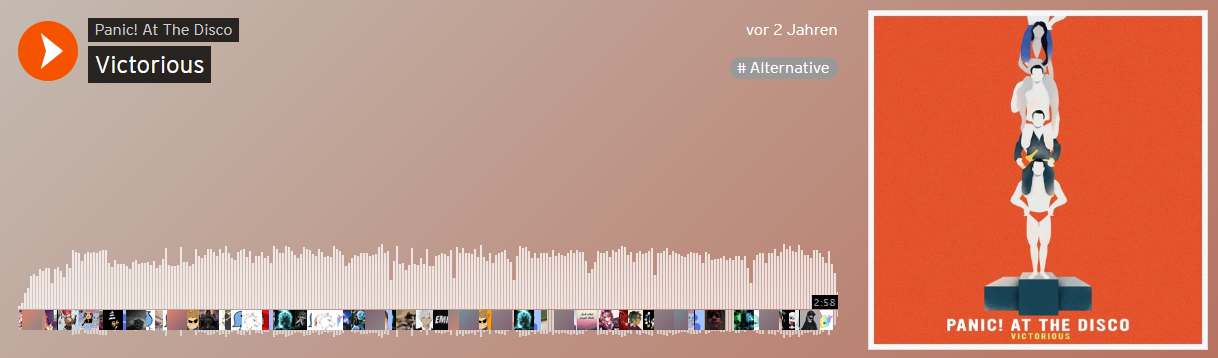
\includegraphics[width=.9\textwidth,center]{SoundCloudPlayer.png}
\caption{\label{fig:SoundCloudPlayer}Player der Musik- und Audio-Plattform \textit{SoundCloud} \citep{SoundCloud2015Panic}}
\end{figure}

\subsubsection{Youtube}
 
Im Bereich der Videoplattformen gilt \textit{Youtube} als die mit Abstand am weitesten verbreitete Videoplattform in Deutschland \citep{statista2016video}.  Zum Abspielen der von den Nutzern hochgeladenen Videos setzt \textit{Youtube} auf den HTML5-Player (siehe Abbildung \ref{fig:YoutubePlayer1}).

\begin{figure}[h!]
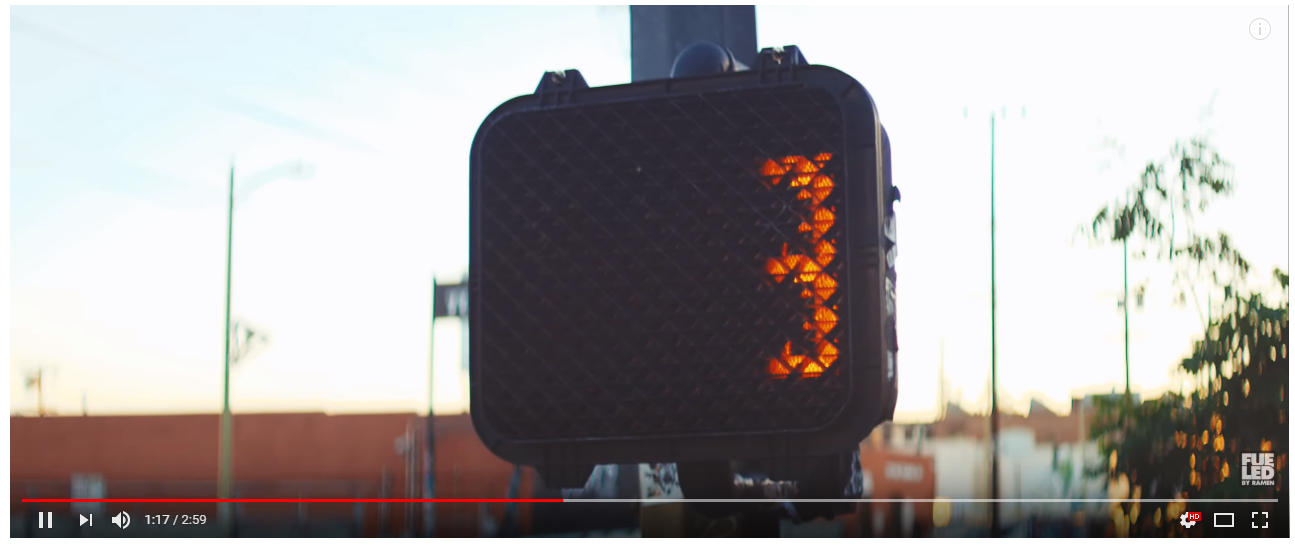
\includegraphics[width=.9\textwidth,center]{YoutubePlayer1.png}
\caption{\label{fig:YoutubePlayer1}Player der Video-Plattform \textit{Youtube} \citep{Youtube2015Panic}}
\end{figure}

In \citep{youtubeinfokarten,youtubeabspann} werden Möglichkeiten aufgezeigt, Informationen an ein Video zu annotieren. Die Informationen können Verweise auf andere Videos, Playlists und Kanäle, eine Abstimmung oder ein Link zu einer genehmigten Webseite beinhalten. Einem Video können insgesamt einen Abspann und bis zu maximal fünf Infokarten mittels des integrierten Webeditors angeheftet werden. Bei Infokarten kann nur der jeweilige Startzeitpunkt für die Anzeige frei festgelegt werden, die Dauer wird durch \textit{Youtube} vorgegeben. In Abbildung \ref{fig:YoutubePlayer2} zeigt, wie eine solche Infokarte im Player dargestellt wird. Ein Abspann kann hingegen nur innerhalb der letzten fünf bis 20 Sekunden eines Videos angezeigt werden.

\begin{figure}[h!]
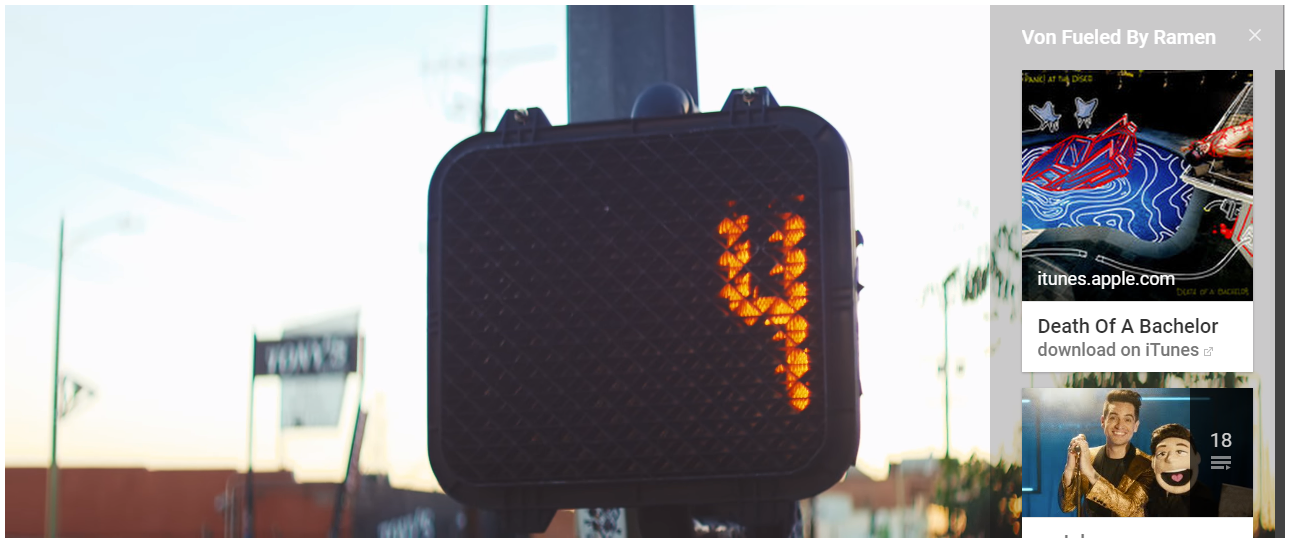
\includegraphics[width=.9\textwidth,center]{YoutubePlayer2.png}
\caption{\label{fig:YoutubePlayer2}Anzeige der Infokarte \citep{Youtube2015Panic}}
\end{figure}


%%%%%%%%%%
\subsection{Technologien für den Einsatz in Moodle}
Bevor mit der Konzeption und Implementierung des Moodle-Plugins begonnen wird, wird sich nun der Analyse der bestehender Komponenten zugewendet, die als Basis für das Plugin dienen können. Ziel ist es festzustellen, ob eventuell bereits Technologien existieren, mit deren Hilfe die Idee des Moodle-Plugins umgesetzt werden kann oder ob zumindest Teile davon - unter entsprechender Beachtung der Lizenzierung - sinnvoll wiederverwendet werden können. Hierbei wird so vorgegangen, dass die einzelnen vorhanden Technologien auf diesem Gebiet und ihre Funktionen vorgestellt und anschließend bewertet werden, inwiefern diese für die Umsetzung des Plugins relevant sind.

\todo[inline]{Um Screenshots ergänzen}
\todo[inline]{sollte nicht auf Moodle bezogen werden. Es bräuchte einen extra Teilabschnitt für Moodle.Plugins.}

%%%%%%%%%%
\subsubsection{VideoJS Player}
Bei dem \textit{VideoJS Player}\footnote{GitHub-Projekt, Apache-Lizenz 2.0: http://videojs.com/; https://github.com/videojs} handelt es sich um eine Open Source Bibliothek zum Abspielen von Videos und stellt damit einen HTML5 Video Player zur Verfügung. Der \textit{VideoJS Player} ist bereits als Standard Plugin für die Wiedergabe von Audio- und Video-Dateien in Moodle integriert. Wie der Name schon erkennen lässt, handelt es sich hierbei um eine JavaSrcipt Bibliothek. Der \textit{VideoJS Player} beschränkt sich in seiner Ausgangsversion ausschließlich auf das Abspielen von Audio- und Video-Dateien und bietet bis auf ein optionales Fallback auf den Adobe FlashPlayer keine weiteren Funktionen. Die Funktionalität des \textit{VideoJS Player} kann aber über Plugins erweitert werden. Es existieren bereits zahlreiche solcher Plugins. Hier sei vor allem das Plugin \textit{videojs-wavesurfer}\footnote{GitHub-Projekt, MIT Lizenz: https://github.com/collab-project/videojs-wavesurfer} zu nennen, welches das wavesurfer.js Framework (siehe Abschnitt \ref{sec:wavesurfer.js}) in den \textit{VideoJS Player} einbindet. Dank der Unterstützung von Plugins ist es durchaus denkbar, den Player mittels Plugin beispielsweise um Buttons zum Erstellen von Kommentaren oder persönlichen Notizen zu erweitern. Auch wäre es denkbar, mittels eines Plugins die annotierten Kommentare zu visualisieren. Grundsätzlich stellt der \textit{VideoJS Player} somit eine gute Ausgangslage für einen Hyperaudio-Player dar.

%%%%%%%%%%
\subsubsection{H5P}
Mit \textit{H5P} und dem bereits vorhanden Plugin für Moodle\footnote{GitHub-Projekt, GNU General Public License v2.0: https://github.com/h5p/h5p-moodle-plugin} ist es möglich, etliche verschieden Arten von interaktiven Lerninhalten zu gestalten. Dabei handelt es sich um eine Sammlung von interaktiven Komponenten, darunter Course Presentation, Timeline und Interactive Video. Course Presentation bietet die Möglichkeit, interaktive Präsentationen zu gestalten. Timeline kann genutzt werden um Inhalte anhand eines Zeitstrahls darzustellen. Interactive Video ermöglicht, ähnlich wie Course Presentation, die Interaktion während des Abspielens eines Videos. Besonders erwähnenswert ist, dass sich bei \textit{H5P} die interaktiven Inhalte innerhalb der Weboberfläche erstellen lassen. Es wäre also denkbar, eine eigene interaktive Komponente zu entwickeln, welche es ermöglicht, Hyperaudio-Dokumente als interaktiven Lerninhalt zu erstellen und abzuspielen.

%%%%%%%%%%
\subsubsection{Popcorn.js}
Die Mozilla Corporation bietet mit \textit{Popcorn.js}\footnote{GitHub-Projekt, MIT Lizenz: https://github.com/mozilla/popcorn-js} eine Bibliothek an, welche neben einer standardisierten Steuerung von Medieninhalten aus verschiedenen Quellen auch die Annotation von Inhalten mittels Plugins ermöglicht. Hier wäre also auch eine Entwicklung eines Plugins denkbar, mit welchem wir Hyperaudio-Dokumente wie gewünscht wiedergeben könnten. Die Wartung für die Bibliothek wurde seitens Mozilla zwar eingestellt, das Projekt steht aber weiterhin auf GitHub zur Verfügung. Obwohl das Projekt nicht mehr weiterentwickelt wird, kann es durch die vorhandenen Steuerungsmöglichkeiten und das Plugin-System ein sehr geeignetes Grundgerüst für die Entwicklung des Moodle Plugins darstellen.
 
%%%%%%%%%%
\subsubsection{wavesurfer.js}
\label{sec:wavesurfer.js}
Bei \textit{wavesurfer.js}\footnote{GitHub-Projekt, BSD-3-Clause: https://wavesurfer-js.org; https://github.com/katspaugh/wavesurfer.js} handelt es sich um ein JavaScript Framework, welches es ermöglicht, die Wellenform zu der abgespielten Audio-Datei in einem Audio-Player visualisieren zu lassen. Diese Basisfunktionalität wurde durch Weiterentwicklungen um nützliche Funktionen erweitert. Auf zwei dieser Weiterentwicklungen gehen wir im Folgenden ein.

%%%%%%%%%%
\subsubsection{audio-annotator}
Der \textit{audio-annotator} stellt eine auf dem \textit{wavesurfer.js} Framework basierende Weiterentwicklung dar, welche es mittels Weboberfläche ermöglicht, Annotationen in Form von Text an eine Audio-Datei anzuheften. Es erweitert \textit{wavesurfer.js} also um die Möglichkeit, Annotationen an eine Datei anzuheften und bietet gleichzeitig noch eine Oberfläche, um ebendiese Annotationen vorzunehmen.

%%%%%%%%%%
\subsubsection{BAT - BMAT Annotation Tool}
Beim \textit{BAT - BMAT Annotation Tool}\footnote{GitHub-Projekt, GNU General Public License 3: https://wavesurfer-js.org; https://github.com/BlaiMelendezCatalan/BAT} handelt es sich um eine Entwicklung basierend auf der im Zusammenhang von \textit{audio-annotator} erweiterten Frameworks \textit{wavesurfer.js} und \textit{regions.js}. Es ermöglicht, ebenso wie \textit{audio-annotator}, dem Benutzer mittels Weboberfläche Annotationen an einer Audio-Datei vorzunehmen. Somit bietet \textit{BAT - BMAT Annotation Tool} logischerweise dieselben Vorzüge wie bereits der \textit{audio-annotator}. Im Vergleich zum \textit{audio-annotator} stellt \textit{BAT - BMAT Annotation Tool} jedoch ein weiterentwickelteres Framework dar.

\todo[inline]{regions.js bereits bei audio-annotator in Verwendung?}

\subsubsection{wavesurfer.js für Hyperaudio-Dokumente}
Das \textit{wavesurfer.js} Framework - speziell mit seinen Weiterenticklungen - bietet einige Funktionen, die für das Abspielen von Hyperaudio-Dokumenten nützlich sein könnten. Zusätzlich bietet es auch die Funktion,  die entsprechenden Annotationen in einer Weboberfläche an die Audio-Dateien anzuheften. Grundsätzlich lässt sich feststellen, dass \textit{wavesurfer.js} und seine Ableger im Vergleich zu den zuvor betrachteten Entwicklungen einen wesentlich unausgereifteren Eindruck hinterlassen.

%%%%%%%%%%
\subsubsection{timesheets.js}
\textit{timesheets.js}\footnote{ehemaliges GitHub-Projekt, MIT Lizenz: http://wam.inrialpes.fr/timesheets} ist ebenfalls ein JavaScript Framemwork, welches analog zu \textit{audio-annotator} und \textit{BAT - BMAT Annotation Tool} die Annotation von zusätzlichen Inhalten ermöglicht. Leider befindet sich das Framework aktuell nicht mehr in der Entwicklung. Aufgrund der Ähnlichkeit zu den {wavesurfer.js} Ablegern und der eingestellten Entwicklung können hier zwar Ideen übernommen werden, als Basis für das zu entwickelnde Moodle-Plugin ist dieses Framework jedoch nicht geeignet.

Zusammenfassend ist festzustellen, dass für die Entwicklung des Plugins für Hyperaudio-Dokumente vor allem \textit{VideoJS Player}, \textit{H5P} und \textit{Popcorn.js} die vielversprechendsten bestehenden Entwicklungen darstellen, da diese bereits einen sehr hohen Entwicklungsstand haben. Unter Anbetracht der benötigten Funktionen stellen aber speziell der \textit{VideoJS Player} und \textit{Popcorn.js} eine sehr gute Basis dar, da diese mit ihrem Kernelement als Player und durch die integrierten Plugin-Systeme für die Entwicklung von Multimedia-Elementen ausgelegt sind. Bei \textit{H5P} müsste die Playerfunktion mit der dazugehörigen Erweiterung für Hyperaudio-Dokumente von Grund auf entwickelt werden, um eine entsprechende interaktive Komponente für Hyperaudio-Dokumente bereitstellen zu können. Letztendlich ist \textit{Popcorn.js} die beste Grundlage für die Entwicklung des Plugins, da hier auch die Steuerung der Medieninhalte bereits von Grund auf ausgeprägt implementiert sind, woraus bei der Umsetzung einiger Funktionen großer Nutzen gezogen werden kann.



%%%%%%%%%%%
%\section{Nutzungsszenarien für das Moodle-Plugin}
%Im nächsten Schritt betrachten wir zunächst die verschiedenen Nutzungsszenarien (auch Usage Scenarios oder Scenarios) unseres Moodle-Plugins. Hierfür wollen wir zunächst den Begriff Usage Scenario definieren.
%
%\glqq Ein Usage Scenario, kurz Scenario, beschreibt anhand eines Beispiels aus der realen Welt, wie eine oder mehrere Personen oder Organisationen mit einem System interagieren.
%Es beschreibt die Schritte, Ereignisse und/oder Aktionen, welche während der Interaktion erfolgen.
%Usage Scenarios können sehr detailliert sein, indem sie genau aufzeigen wie jemand mit der Benutzeroberfläche arbeitet, oder lediglich sehr oberflächlich, wenn nur die kritischen Geschäftsaktionen beschrieben werden, aber nicht wie diese ausgeführt werden\grqq{} \citep{agilemodeling2018stat}.
%
%%A usage scenario, or scenario for short, describes a real-world example of how one or more people or organizations interact with a system. They describe the steps, events, and/or actions which occur during the interaction. Usage scenarios can be very detailed, indicating exactly how someone works with the user interface, or reasonably high-level describing the critical business actions but not the indicating how they're performed.
%
%Für die Konzeption des Plugins macht es Sinn, Nutzungsszenarien aus den verschiedenen Perspektiven zu betrachten, in unserem Fall aus Sicht der Lehrenden und der Studierenden.

%%%%%%%%%%
\section{Zusammenhänge der Komponenten von Hyperaudio-Dokument und Annotationen}
Basierend auf der Definition eines Hyperaudio-Dokuments aus Abschnitt \ref{sec:hyperaudio} und der in Abschnitt \ref{sec:anforderungsdefinition} erarbeiteten Anforderungen werden die Zusammenhänge der medialen Komponenten weiter analysiert. Hierbei soll vor allem geklärt werden, wie die einzelnen Komponenten von Hyperaudio-Dokument und Annotationen zusammenhängen und welche Möglichkeiten dadurch gegeben beziehungsweise nicht gegeben sind.

\todo[inline]{Gehört das nicht zum Konzept? Immerhin erklären Sie die Entitäten und Beziehungen von den Komponenten.}

%%%%%%%%%%
\subsection{Komponenten}
Im Mittelpunkt eines Hyperaudio-Dokuments steht eine Audio-Datei. Inhaltlich kann es sich hierbei beispielsweise um einen Vorlesungsvortrag handeln. Man könnte sich auch vorstellen, dass ein Hyperaudio-Dokument aus mehreren aneinandergereihten Audio-Dateien besteht. Dies würde an der grundsätzlichen Problemstellung jedoch nichts ändern und kann im Nachhinein jederzeit als Erweiterung umgesetzt werden. Aus diesem Grund wird in dieser Arbeit nur ein Plugin für ein Hyperaudio-Dokument bestehend aus einer Audio-Datei entwickelt.

Neben dieser zentralen Audio-Datei besteht das Hyperaudio-Dokument aus mehreren Zusatzinhalten, wobei es sich um Bilder, Graphen, Tabellen usw. handeln kann. Entscheidend ist aber, dass diese Zusatzinhalte immer nur eine rein grafische Darstellung verkörpern. Videos mit Ton sind somit beispielsweise nicht als Zusatzinhalt verwendbar, reine Animationen ohne Ton sind aber durchaus möglich.

Als besondere, nämlich externe Komponente, sind die Kommentare zu nennen. Diese gehören nicht zum eigentlichen Hyperaudio-Dokument, sollen aber mit diesem verknüpft werden. Es wird drei verschiedene Arten von Kommentaren geben, nämlich  öffentliche Kommentare, persönliche Notizen und persönliche Markierungen. Innerhalb der öffentlichen Kommentare muss noch zwischen den Original-Kommentaren und den Antworten auf diese unterschieden werden. 


%%%%%%%%%%
\subsection{Zusammenhänge}
\label{sec:komponenten_zusammenhänge}
Diese Zusammenhänge der soeben genannten Komponenten sind im UML-Diagramm in Abbildung \ref{fig:UMLAufbau} ersichtlich. Zunächst werden die Zusammenhänge zwischen der Audio-Datei und den Zusatzinhalten betrachtet. Zu jedem beliebigen Zeitpunkt innerhalb der Abspieldauer der Audio-Datei kann maximal ein Zusatzinhalt gleichzeitig annotiert werden. Es sind also auch Phasen möglich, zu denen keinerlei Zusatzinhalt dargestellt wird. Das Zeitfenster für die Annotation soll mittels einer Start- und Endzeit pro Zusatzinhalt definiert werden, wobei nur die Minuten und Sekunden anzugeben sind. Bei dem Zeitfenster sollte natürlich bedacht werden, dass dieses nicht zu kurz sein sollte. Zwar soll, sobald ein Zusatzinhalt im Player des Hyperaudio-Dokuments angezeigt wird, ein entsprechender Audio Cue abgespielt werden, dennoch können bereits einige Sekunden vergehen bis der Studierende seinen Blick dem Player zuwendet.

Auch die Kommentare stehen als externe Komponente in einer gewissen Art und Weise im Zusammenhang mit der Audio-Datei. Dies ergibt sich daraus, dass Kommentare zu einem bestimmten Zeitpunkt innerhalb der Audio-Datei erfasst werden. Während Antworten auf Original-Kommentare erfasst werden können, sind Antworten auf Antworten nicht möglich.

\todo[inline]{Master-Slave-Prinzip. Es gibt ein Führungsmedium und mehrere abhängige Medien.}

Zwischen Kommentaren und Zusatzinhalten gibt es jedoch keinen direkten Zusammenhang. Solche Zusammenhänge ergeben sich alleine aus den Zeitpunkten der Annotationen. Zusatzinhalte können wiederum in keinem Zusammenhang mit einem anderen Zusatzinhalt stehen.


\begin{figure}[h!]
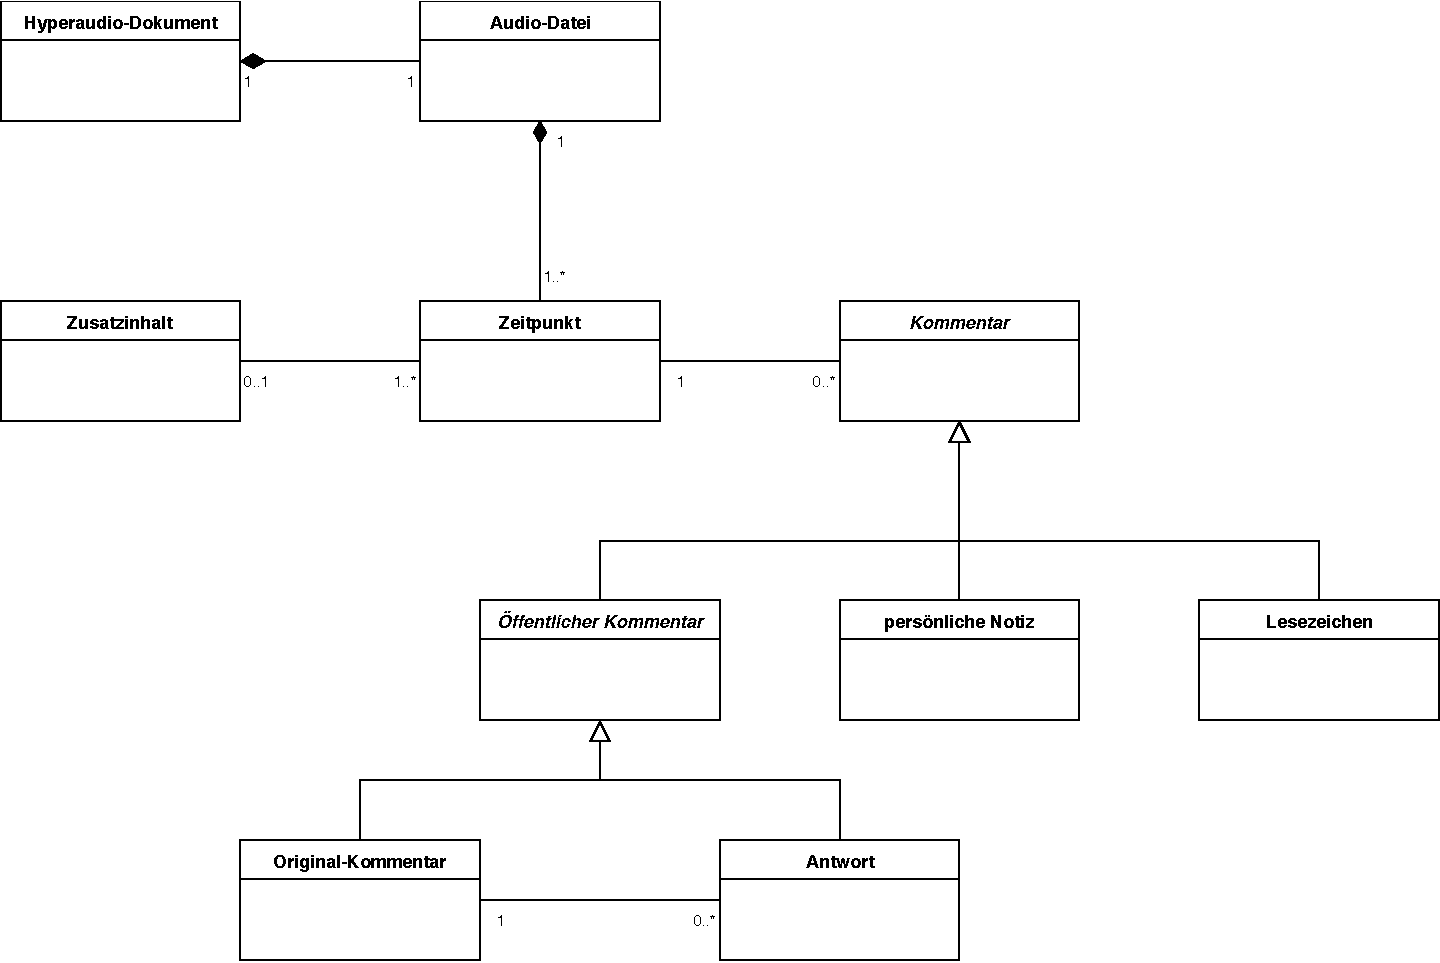
\includegraphics[width=\textwidth,center]{UMLZusammenhaenge.pdf}
\caption{\label{fig:UMLAufbau}Zusammenhänge der Komponenten}
\end{figure}

%%%%%%%%%%
\section{Zusammenfassung}
\dots
